\documentclass[twocolumn]{article}

\usepackage[english]{babel}

\usepackage{graphicx}
\graphicspath{{figs/}}


\usepackage{tikz}
\usetikzlibrary{shapes}

\usepackage{subcaption}

\usepackage[draft]{fixme}

\newcommand{\ie}{{\textit{i.e.\ }}}
\newcommand{\cf}{{\textit{cf\ }}}
\newcommand{\eg}{{\textit{e.g.\ }}}
\newcommand{\al}{{\textit{et al.\ }}}

\newcommand{\M}[3]{{\mathcal{M}(#1, #2, #3)}}
\newcommand{\model}[3]{{$\mathcal{M}(#1, #2, #3)$}}
\newcommand{\refmodel}[2]{{$\mathcal{M}(#1, #2)$}}
\newcommand{\Model}[3]{{$\mathcal{M}^{\circ}(#1, #2, #3)$}}

\newcommand{\groundingcriterion}{{$\mathcal{M}^{\circ}_{min}$}}
\newcommand{\inigrounding}{{$\mathcal{M}^{\circ}_{t_0}$}}

\newcommand{\concept}[1]{{\small \texttt{#1}}}
\newcommand{\stmt}[1]{{\footnotesize \tt $\langle$ #1\relax$\rangle$}}


\title{Is Partner Modeling Mutual?}

\begin{document}
\maketitle

\begin{abstract}
    TDB
\end{abstract}

\section{Introduction}


From its very beginning, CSCL research has been following Roschelle \& Teasley's
(1986) suggestion that collaborative learning has something to do with the
process of constructing and maintaining a shared understanding of the task at
hand. Building a shared/mutual understanding refers to the upper class of
collaborative learning situations, those in which students should build upon
each other's understanding to refine their own understanding. What is expected
to produce learning is not the mere fact that two students build the same
understanding but the cognitive effort they have to engage to build this shared
understanding (Schwartz, 1995). This effort can be observed by the frequency of
rich interactions, i.e. interactions whose occurrence has been related to
learning: (self-) explanations in cognitive science (Chi ; Webb), conflict
resolution in socio-cognitive theories (Doise), mutual regulation (Blaye,) in a
Vygostkian perspective, etc. The construction of a shared understanding has been
investigated for several years in psycholinguistics, under the  notion of
“grounding” (Clark \&Wilkes-Gibbs, 1986). However, the relevance of grounding
mechanisms for explaining learning outcomes has been questioned. The monitoring
and repair of mis-understanding explains for instance referential failures in
short dialogue episodes but does hardly predict conceptual change over longer
sessions (Dillenbourg \& Traum, 2006). The cumulative effect of grounding
episodes can probably be better understood from a socio-cultural perspective:
"collaborative learning is associated with the increased cognitive-interactional
effort involved in the transition from learning to understand each other to
learning to understand the meanings of the semiotic tools that constitute the
mediators of interpersonal interaction" (Baker, Hansen, Joiner \& Traum, 1999).
Several scholars suggest that CSCL research should go deeper in the
understanding of how partners engage into shared meaning making (Stahl, 2006) or
'intersubjective' meaning making (Suthers (2006).  

Paradoxically, while Clark's theory is somewhat too linguistic from a conceptual
change viewpoint, it is criticized at the same time as being too cognitivist by
some psycholinguists, i.e. as overestimating the amount shared knowledge and
mutual representations actually necessary to conduct a dialogue. The fundamental
issue, as old as philosophy, is the degree of coupling between the different
levels of dialogue, mostly between the lexical / syntactical level and the
deeper semantic levels. Pickering \& Garrod (2004) argue that the mutual
understanding starts mostly with a 'local alignment' at the level of the
linguistic representations, due to priming mechanisms, and that this superficial
alignment may – in some cases- lead to a 'global alignment' of the semantic
level.  For these authors, the convergence in dialogue, and even the repair of
some misunderstandings, is explained by this mimetic behavior more than by a
monitoring of each other's knowledge: "…interlocutors do not need to monitor and
develop full common ground as a regular, constant part of routine conversation,
as it would be unnecessary and far too costly. Establishment of full common
ground is, we argue, a specialized and non-automatic process that is used
primarily in times of difficulty (when radical misalignment becomes apparent)."
(p. 179). This view is actually not incompatible with Clark's grounding
criterion (REF): the degree of shared understanding that peers need to reach
depends upon the task they perform. For instance, a dialogue between two
surgeons might rely on superficial alignment if they talk about their friends
but has to guarantee accurate common grounds when talking about which
intervention will be conducted in which way on which patient.  Some CSCL
scholars stressed the 'illusion of shared understanding' (JACCO?), i.e. the
potential decoupling between linguistic alignment and actual shared meanings.

This interesting cognitive science debate mostly occurred outside the field of
learning. In education, the question is to relate these mechanisms to learning
outcomes. Is linguistic alignment sufficient to trigger conceptual change? Does
negotiation of meaning only occurs when partners monitor and diagnose each
other's knowledge. If the ratio between shallow alignment and deep grounding
depends upon the task, and if deep grounding is a condition for learning, then
the pedagogical challenge is to design tasks that require deep grounding. Most
empirical studies on grounding and alignment are conducted with tasks, which
despite being qualified as 'ecologically valid' by their authors, are mere
referencing tasks such as asking the way to the train station or helping the
peer to choose a picture among many. In this contribution, we explore several
richer tasks such as arguing on a sensitive issue or building a concept map.  

Deep grounding or shared meaning making requires some cognitive load. For Clark
\& Wilkes-Gibbs (1986), what is important is not the individual effort made by
the receiver of a communicative act, but the overall least collaborative effort.
The cost of producing a perfect utterance may be higher than the cost of
repairing the problems that may arise through misunderstandings. For instance,
subjects are less careful about adapting their utterances to their partner when
they know they can provide feedback on his/her understanding (Schober, 1993). We
introduced the notion of ‘optimal collaborative effort’ (Dillenbourg et al,
1996) to stress that misunderstanding should not be viewed as something to be
avoided (if this was possible), but as an opportunity to engage into
verbalization, explanation, negotiation, and so forth. This issue is related to
the global argument regarding cognitive load in learning activities, especially
in discovery learning environments: there is no learning without some cognitive
load, but overload may hinder learning (Paas, Renkl \& Sweller, 2003). In the
context of collaborative learning, we understand the cognitive load induced by
mutual modeling as part of Schwartz’s (1995) notion of effort towards a shared
understanding. For instance, CSCL researchers expanded the use of 'collaboration
scripts' (Aronson,?). A script is a pedagogical method that collaborative
learning activities in order to foster the emergence of productive interactions
such as argumentation, explanation or conflict. Conflict-resolution scripts such
as the ArgueGraph (Dillenbourg \& Hong, 2008) forms pair of students with
opposite opinions, which increases the difficulty of consensus building,
requiring more justifications, more negotiation, more load. Similarly, JIGSAW
scripts provide peers with different but complementary knowledge for augmenting
(reasonably) the effort group members have to engage to reach a shared solution. 

%\paragraph{Theory of Mind}
%
%Theory of Mind (originally defined in~\cite{premack1978does}) is the cognitive
%ability that a subject possesses to represent the mental state of another
%agent, possibly including knowledge that contradicts the subject's own model: for
%example, a book can be at the same time \emph{visible} for myself, and \emph{not
%visible} for you.
%
%Children develop this skill, which is essential to understand others'
%perspectives during interactions, around the age of three. It supposes the
%ability to build, store and retrieve separate models of the knowledge of the
%interactors.
%
%One classical application of this cognitive skill is the so-called
%\emph{False-Belief} experiment (also known as the \emph{Sally and Ann}
%experiment)~\cite{Leslie2000}: a child is asked to watch a scene where two
%people, A and B, manipulate objects. Then A leaves and B hides away one
%object. When A comes back, we ask the child ``where do you think A will
%look for the object?''. Before acquiring a theory of mind, children are not
%able to separate their own (true) model of the world (where they know that
%the object was hidden) from the model of A, which contains \emph{false
%beliefs} on the world (A still thinks the object is at its original
%position since he did not see B hiding it).

\section{Mutual Modeling}


In order to build a shared understanding, do partners have to build a
representation of each other's knowledge? We refer to \emph{mutual modeling} as
the process of inferring one's partner mental states. Any claim that students
carry out a detailed monitoring of their peers would be as incorrect as any
claim that they do not maintain any representation at all. If mutual modeling
had to be permanently detailed and accurate, subjects would obviously face a
huge cognitive load. Conversely, peers could not collaborate without some
minimal amount of mutual modeling. For instance, A cannot disagree with B
without knowing that B has a different opinion. The mutual model can be implicit
(A is not aware of what he knows about B), by-default (I believe that B beliefs
what I believe unless contrary evidence), opportunistic (A does not model B
unless the conversation requires it), global (A infers B's beliefs based on
categories such as age, culture or profession) and, of course, it can be
incorrect… but it can not remain empty. Dialogues include many instances of
utterances such as "I thought he would do that" (first level of mutual
modelling) or even "He thought I would do that but I intended something else."
(second level of mutual modelling).

The content of mutual models ranges from 'dispositional' versus 'situational'
aspects. The 'dispositional' aspects refer to A's representation of B's long
term knowledge, skills or traits. It is thus closely related to the notion of
transactive memory~\cite{wegner1987transactive, moreland1999transactive}.
'Situational' aspects refer to A's representation of B's knowledge, behavior or
intentions specifically activated in the situation in which A and B are
collaborating, some of them being valid for 2 seconds, other ones for 2 hours.
Here are examples of fragments that constitute A's model of B regarding to
aspects X, noted $Model(A,B,X)$:

\begin{itemize}

    \item $Model(A,B, knowledge)$: What does A know about B's knowledge with
        respect to the task at hand or, inversely, about B's knowledge gaps?
        When can A consider B's statements as reliable? 

    \item $Model(A,B, skills)$: What does A know about B's skills with respect to
        the task at hand? May A expect B to perform well in a specific subtask?
        The effectiveness of division of labor depends on the quality of this
        mutual model. 

    \item $Model(A,B, goals)$: What does A know about B's intentions with respect
        to the project, including B' motivation and commitment? Can A trust B
        when B promises to deliver? 

    \item $Model(A,B, task)$: What does A know about B's representation of the
        situation and the task: does A knows whether B has the same
        understanding of the problem at stake? 

    \item $Model(A,B, plans)$: What does A know about B's strategy. Does A
        understand why B did what he did? Is A able to anticipate what B will do
        next? 

    \item $Model(A,B, "urgent")$: What does A about know B's understanding of A's
        last utterance: does ‘urgent’ means now, ASAP and ‘not too lat’ ?

    \item We could continue the list of what is X is \model{A}{B}{X}: beliefs,
        emotions, history, status, …

\end{itemize}

We have different levels of mutual modelling. If A states "B thinks I am god in maths", we
are the second level of mutual modelling:  $Model(A, B, Model(B,A, knowledge="good in
math"))$. There is an infinite regress of nested models: If A says "B knows that
I don't expect him to solve this statistics problem" corresponds to $Model(A, B,
Model (B, A (Model (A,B, statistic-skills)))$.

A partner model is probably not a "box", \ie not a monolithical representation
but rather a mosaic of information fragments about the partner, with various
grain sizes and various life cycles. This mosaic is elaborated through various
mechanisms, first for building an initial model of the partner and then for
updating this model.  As two students meet for the first time, mutual models are
initialized by the assumptions they make upon each other from cues such as
his/her membership to large categories (age, culture, profession, ...) include
stereotypes (sportsmen, junkie, business women, Swiss,...) as well as physical
appearance. Scholars studied how initial modeling impacts communication. In
their experiments on initial mutual modelling, Slugoski, Lalljee, Lamb \&
Ginsburg~\cite{slugoski1993attribution} pretended to their subjects that their
(fake) partner had or had not received the same information. They observed that
the subjects adapted their dialogue by focusing the explanation on the items
that (s)he was supposed to ignore. Brennan (1991) \fixme{ref} showed that the subjects used
different initial strategies in forming queries depending on who they were told
their partner was.  

Initial common grounds are also initiated by co-presence: they include events to
which A and B attended together~\cite{clark2002definite} in the physical space
or in our cultural space (\eg ‘09-11’). Co-presence means that we can refer to
a shared objects and event,-s it does of course not imply that we give them the
same meaning. Namely, a shared screen does not mean a shared
understanding~\cite{dillenbourg2006sharing}.

After initialization, mutual models are updated along the collaborative work
through verbal and non-verbal interactions. A default inference rule is that "my
partner agrees with me unless he disagrees", which reject the critiques that
mutual modeling generates an unbearable cognitive load. This default rule is
superseded by the several mechanisms for monitoring and repairing one's partner
understanding: acknowledgement, continuous attention, relevance of next turns,
facial expressions including gaze signals, etc.

Mutual modeling does not occur in a vacuum but it is highly contextualized. REF
reviews the features of the collaborative situation, namely the media
(cotemporality… ), may facilitate or hamper mutual modeling. Hutchins (SILENCE)
reported a study in which a short silence between two pilots was perfectly
interpreted because it occurred in a highly constrained communication context.
Some environments are more productive than others in helping peers to detect
their misunderstandings. Roschelle~\cite{roschelle1995construction} reformulate
the design of CSCL interfaces as providing ways for peer to detect and repairs
their misunderstanding. In CSCW, researchers have explored various so-called
"awareness tools", \ie functionalities that inform A is about B's actions that A
could not directly perceived because B was working on a different subset of the
virtual space. Different awareness tools will be addressed in this contribution
since they allowed us to manipulate experimentally the mutual modelling activity. 


%\subsection{State of the Art}
%
%\paragraph{Building a model of a human during the interaction} Perspective
%Taking is a human ability which allows one to put him/herself in another
%person's point of view. Studied in psychology
%literature~\cite{Flavell1992,Tversky1999}, this ability is crucial when
%interacting with people by allowing one to reason on others' understanding of
%the world in terms of visual perception, spatial descriptions, affordances and
%beliefs, etc.  In the last years these notions have been gradually employed in
%HRI.~\cite{Breazeal2006} presents a learning algorithm that takes into account
%information about a teacher's visual perspective in order to learn a task.
%~\cite{Johnson2005} apply visual perspective taking for action recognition
%between two robots.~\cite{Trafton2005} use both visual and spatial perspective
%taking to find out the referent indicated by a human partner.
%
%The cognitive model that the robot builds for the agent it interacts with is
%still simple and mostly focused on geometric features (who sees what? What are
%our relative positions? etc.). Extending this knowledge with more subtle
%perceptions (emotional state for instance) remains to be done.
%
%\paragraph{Joint action}
%Several theories dealing with collaboration~\cite{Cohen1991,Grosz1996,Clark1996}
%emphasize that collaborative tasks have specific requirements compared to
%individual ones, \eg, since the robot and the person share a common goal, they
%have to agree on the manner to realize it, they must show their commitment to
%the goal during execution, etc. Several robotic systems have already been built
%based on these theories~\cite{Rich1997,Sidner2005,Breazeal2003} and they all
%have shown benefits of this approach. They have also shown how difficult it is
%to manage turn-taking between communication partners and to interleave task
%realization and communication in a generic way. Finally, today only few
%systems~\cite{Fong2006,Breazeal2003,Sisbot2008} take humans into account at all
%levels.
%
\section{A model for mutual modelling evaluation}

To report experiments on mutual modeling, we suggest
the notation \model{A}{B}{X} to denote ``A knows that B knows X". This is a
simple but useful reduction to reason on mutual modelling. This
notation does not mean A has an explicit, monolithic representation of B: it
must be understood as an abstraction referring to complex socio-cognitive
processes. Besides, we refer to the \emph{degree of accuracy} of the model as
\Model{A}{B}{X}.

We parametrize and assess the mutual modelling effort through 3 variables:

\begin{enumerate}

    \item Tasks vary a lot with respect to how much they require.  The grounding
        criterion -- denoted \groundingcriterion -- refers to how
        important it is to mutually share a piece of information X to succeed
        the task T. It can be computed as the probability to succeed T despite
        the fact X is not grounded. $\mathcal{M}^{\circ}_{min}(A,B,X)$ can be
        estimated from the correlation between \Model{A}{B}{X} and task
        performance. 

    \item Before any specific grounding act, there is usually a non-null probability
        that X is mutually understood by A and B: because X is part of A's and
        B's cultures, because it is manifest to co-present subjects or simply
        because there is not much space for misunderstanding or disagreement
        about X. We could not simply collaborate without a high level of initial
        grounds. We note the theoretical accuracy of initial grounds:
        $\mathcal{M}^{\circ}_{t_0}(A,B,X)$.

    \item The cost of grounding X refers to the physical and cognitive effort
        necessary to perform a grounding act $\alpha$: a verbal repair (\eg
        rephrasing), a deictic gesture, a physical move to adopt one partner's
        viewpoint, etc. This cost varies according to media features ( Clark \&
        Brennan (REF)). 

\end{enumerate}

Based on these 3 parameters, the probability of making an action $\alpha_{t_1}$ about
content X at time $t_1$ during task T in order to increase \Model{A}{B}{X}
at time $t_2$ is the ratio between how much it is needed  ((2)-(1)) and how much it
costs (3)~\cite{traum1996miscommunication}:

\begin{equation} \label{eq:probrepair}
p(\alpha_{t_1}(X,T) / M^{\circ}_{t_2}(A,B,X) \nearrow) \approx \frac{(M^{\circ}_{min}(A,B,X,T) -
M^{\circ}_{t_1}(A,B,X))}{cost (\alpha)}
\end{equation}

This is qualitative summary more that a real equation since several parameters
are hard to quantify (\eg the cost an communication acts depends upon the user
as well) but it clarifies the parameters of the experiments we propose hereafter.

\begin{itemize}
    \item \Model{A}{B}{X}: Our experiments address different contents that can be
        represented in mutual models:

    \begin{enumerate}
        \item \model{A}{B}{emotion}: how accurately A perceives B's emotional state
            (study 3); 

        \item \model{A}{B}{actions} is about how well A guesses what action B has
            done (study 2) or will do next  (study 1)

        \item \model{A}{B}{knowledge}: how accurately A estimates B's knowledge
            with respect to the material they learn together (study 4 and 5)

    \end{enumerate}



    \item \Model{A,B}{X}{T} Our studies concern various collaborative tasks:
        argumentation (study 3), games (study 1 and 2) and concept mapping
        (study 4 and 5). By varying the tasks, we do actually vary the grounding
        criterion but they all require a "reasonably high" grounding criterion.
        All tasks are about building a solution or a representation together; we
        did not address everyday conversations. 

    \item $\mathcal{M}^{\circ}_{t1}(A,B,X)$ Along the same reasoning, the initial degree
        of common grounds should be rather low (and hence the difference between
        initial and required degrees rather high) in order to make mutual
        modelling effort more observable. Studies 1, 4 and 5 have been conducted
        with teams of students who did not know each other. They came
        nonetheless from the same university: they hence had some general common
        grounds.  For studies 2 and 3, students knew each other before for
        reasons explained later on. In study 5, we manipulated the initial mutual modelling by
        using a JIGSAW script.

    \item $cost(\alpha)$ In all studies but study 4, the cost of  grounding is
        an independent variable. Study 3 uses media richness as independent
        variable, with the hypothesis that modeling emotions is "cheaper" with a
        richer medium, \ie  when peers can see each other.  Studies 1,2 and 4
        use awareness tools which, in principle, reduce the cost of mutual modelling, but do
        not eliminate all costs: if the tool provide A with information about
        what B does/knows, this additional information may actually increase
        cognitive load. Awareness tools constitute as a kind of mutual modelling prosthesis,
        and, like any prosthesis, they many augment mutual modelling (by facilitating it or
        even scaffolding it) or inhibit it (by making it useless).

\end{itemize}


Each of the studies that we present in the next section have been design in such a way that, while tractable on a
robot, mutual modelling plays a key role for the task performance: the tasks
require a ``reasonably high" grounding criterion \groundingcriterion,
and all tasks are about building a solution or a representation together.

Along the same reasoning, the initial degree of common grounds \inigrounding
should be rather low (and hence the difference between initial and required
degrees rather high) in order to make mutual modelling effort more observable.
While we can exactly control the actual initial knowledge available to the
robot, estimating \inigrounding still requires special care during the design of
the experiments: as we have previously shown~\cite{lemaignan2014dynamics,
lemaignan2014cognitive} and because the interaction takes place between a human and
a robot, the initial human model of the robot can widely vary depending on
several factors like the user familiarity with technology, the effect of
novelty, the user expectations or the anthropomorphic features of the robot.

More generally, while we have explicit access to \model{R}{H}{X} (from the facts
stored in the robot belief state, as illustrated in
Table~\ref{table|beliefsfig7}), estimating \Model{R}{H}{X} also requires
\model{H}{H}{X}, which depends on the meta-cognitive competencies of the human
partner.

Conversely, measuring \Model{A}{B}{X} is methodologically difficult. We
discriminate two steps, first to capture \model{A}{B}{X} and then to
estimate \Model{A}{B}{X}. 

\begin{itemize}
    \item {\bf Capturing \model{A}{B}{X}}: The simplest method is to ask $A$ what (s)he
        believes about what $B$ knows, feels, intends to do, etc. This raises
        obvious methodological concerns since such a question triggers a
        modeling process beyond what it would 'naturally' be. To avoid this
        bias, one can estimate mutual modeling after task completion. Then, the
        obvious drawback are memory losses and by post-hoc reconstruction.
        The first method was used in study 2 and the
        second one in the other studies. Another option would be to rely on external behavioural metrics like
        eye-tracking: we hypothesise for instance that the fixation time
        reflects the efforts engaged by the human to understand, hence, model,
        the others. Such an approach has however not yet been investigated in the presented studies.

    \item {\bf Estimating \Model{A}{B}{X}}: Once \model{A}{B}{X} is captured, we
        need to access the reference model \refmodel{B}{X} to estimate its
        \emph{accuracy}. Since we can only indirectly access it via what $B$
        reports (\ie \model{B}{B}{X}), accuracy can be estimated in 2 ways:

        \begin{itemize}

            \item Subjective accuracy: In study 3, we compute
                \Model{A}{B}{X} by measuring if $A$ describes
                $B$'s emotions in the same way $B$ reports its emotions 
                ($\M{A}{B}{X} = \M{B}{B}{X}$).

            \item Objective accuracy: In studies 4 and 5, we compute
                \Model{A}{B}{X} by comparing \Model{A}{B}{K} to $B$'s
                actual knowledge as it has measured by a test.

        \end{itemize}

\end{itemize}


\subsubsection{Studies}

The experiments we report here address mutual modelling across different tasks, some with
dyads, other with triads. They were conducted along 6 years in two different
institutions by different researchers. They used different independent,
intermediate and dependent variables. Nonetheless, we were able to address a few
questions across these studies. We start with 3 simple hypotheses about
$\mathcal{M}^{\circ}(A,B)$:

\begin{itemize}
    \item $\mathcal{H}_{1}$: $\mathcal{M}^{\circ}(A,B)$ depends upon A's ability or effort
        to model B,
    
    \item $\mathcal{H}_{2}$: $\mathcal{M}^{\circ}(A,B)$ depends upon  B's ability of
        effort to help A to model him/herself 

    \item $\mathcal{H}_{3}$: $\mathcal{M}^{\circ}(A,B)$ depends upon the quality of
        interactions among A and B

\end{itemize}



$\mathcal{H}_{2}$ is also called a second level modeling hypothesis since H
needs to monitor B to see if A understood him/her
$\mathcal{M}(B,(A,\mathcal{M}(A,B)))$

Our main issue is the symmetry questions: what is the relationship
(Fig.~\ref{mm_symmetry}) between \Model{A}{B}{X} and
\Model{B}{A}{X}? A low symmetry would mean that mutual modeling is
mainly an individual attitude/aptitude ($\mathcal{H}_{1}$). A high correlation
might support $\mathcal{H}_{2}$ since there is a low probability that randomly
formed pairs integrate peers with the same level of mutual modelling skills.

\begin{figure}[htb]
\centering

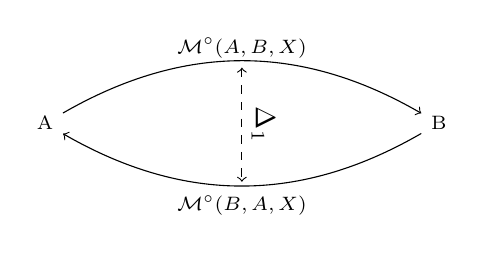
\begin{tikzpicture}[scale=0.5]

\draw(0,0) node[anchor=north] (A) {\scriptsize A};
\draw(10,0) node[anchor=north] (B) {\scriptsize B};
\draw(5,2) node[anchor=north] {\scriptsize \Model{A}{ B}{ X}};
\draw(5,-2) node[anchor=north] {\scriptsize \Model{B}{ A}{ X}};
\draw[dashed, <->] (5,1) -- (5,-1.9) node[midway, sloped, above] {$\Delta_1$};
\draw[->] (A) to[bend left] (B);
\draw[->] (B) to[bend left] (A);

\end{tikzpicture}

\caption{The mutual modelling symmetry question $\Delta_1 =  \Delta(\mathcal{M}^{\circ} (A,B,X),
\mathcal{M}^{\circ} (B,A,X))$}

\label{mm_symmetry}
\end{figure}


With triads, we may compute the accuracy of 6 models:
\Model{A}{B}{X}, \Model{B}{A}{X}, \Model{A}{C}{X}, \Model{C}{A}{X},
\Model{C}{B}{X} and \Model{B}{C}{X}. This enables two
triangle questions (see Fig.~\ref{mm_triangles}):

Do A and B have the same accuracy when modeling C? $\Delta_2 =
\Delta(\M{A}{C}{X}, \M{B}{C}{X})$ If it is the same,
$\mathcal{H}_{2}$ and $\mathcal{H}_{3}$ gain over $\mathcal{H}_{1}$

Does C model more accurately A than B? $\Delta_3= \Delta(\M{C}{A}{X},
\M{C}{B}{X})$ A positive answer would support $\mathcal{H}_{3}$.

\begin{figure}[htb]
\centering
\subcaptionbox{}{ 
    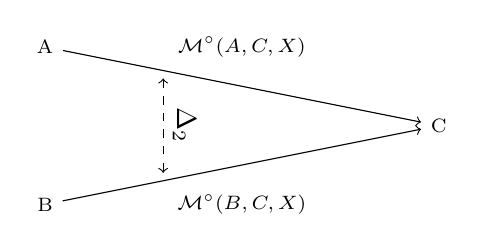
\begin{tikzpicture}[scale=0.5]

    \draw(0,2) node (A) {\scriptsize A};
    \draw(0,-2) node (B) {\scriptsize B};
    \draw(10,0) node (C) {\scriptsize C};

    \draw(5,2) node {\scriptsize \Model{A}{ C}{ X}};
    \draw(5,-2) node {\scriptsize \Model{B}{ C}{ X}};
    \draw[dashed, <->] (3,1.2) -- (3,-1.2) node[midway, sloped, above] {$\Delta_2$};
    \draw[->] (A) to (C);
    \draw[->] (B) to (C);

    \end{tikzpicture}
}
\subcaptionbox{}{ 
    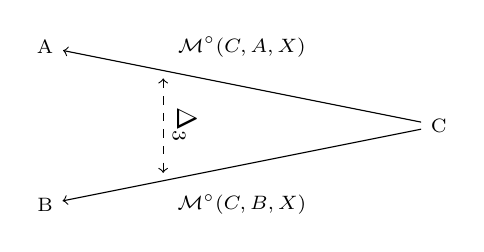
\begin{tikzpicture}[scale=0.5]

    \draw(0,2) node (A) {\scriptsize A};
    \draw(0,-2) node (B) {\scriptsize B};
    \draw(10,0) node (C) {\scriptsize C};

    \draw(5,2) node {\scriptsize \Model{C}{ A}{ X}};
    \draw(5,-2) node {\scriptsize \Model{C}{ B}{ X}};
    \draw[dashed, <->] (3,1.2) -- (3,-1.2) node[midway, sloped, above]
    {$\Delta_3$};
    \draw[<-] (A) to (C);
    \draw[<-] (B) to (C);

    \end{tikzpicture}
}
\caption{The mutual modelling triangle questions}

\label{mm_triangles}
\end{figure}



In addition, the comparison between $\Delta_2$ and $\Delta_3$ could tell us
whether the accuracy of mutual modelling depends more upon the modeller's effort
or the modellee's behaviour.

\paragraph{The rectangle questions}

We could go further by comparing self- versus other modeling $\Delta_4$ in
Fig.~\ref{mm_rectangle}) as an indication of metacognitive skills. We could also
see if modeling skills depend upon what aspects are being modeled (X or Y),
which would explain vertical differences ($\Delta_5$ in
Fig.~\ref{mm_rectangle}). We do not further develop these questions because we
don’t have the necessary data in our studies.

\begin{figure}[htb]
\centering

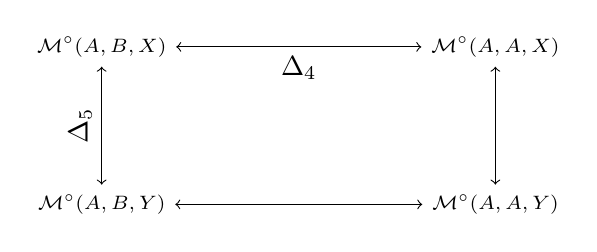
\begin{tikzpicture}[scale=0.5]

    \draw(0,0) node (a) {\scriptsize \Model{A}{ B}{ X}};
    \draw(10,0) node (b) {\scriptsize \Model{A}{ A}{ X}};
    \draw(10,-4) node (c) {\scriptsize \Model{A}{ A}{ Y}};
    \draw(0,-4) node (d) {\scriptsize \Model{A}{ B}{ Y}};
    \draw[<->] (a) -- (b) node[midway, below] {$\Delta_4$};
    \draw[<->] (b) -- (c);
    \draw[<->] (c) -- (d);
    \draw[<->] (d) -- (a) node[midway, sloped, above] {$\Delta_5$};

\end{tikzpicture}

\caption{The rectangle questions}

\label{mm_rectangle}
\end{figure}


This simple notation does not pretend to provide a mathematical account of
mutual modeling but to be more systematic in describing the following
experiments. 

\section{Studies}

\subsection{Study 1: Effect of an awareness tool on \Model{A}{B} in a virtual
game}

\paragraph{Questions}

We studied the impact of an awareness tool on group performance and mutual
modeling. (Nova, Wehrle, Goslin, Bourquin \& Dillenbourg (2006). The availability
of an awareness tool was our independent variable. In previous studies, we
replayed a video of the game to subjects who surprised us by their ability to
remember former states of their mutual model: "I did that because I thought that
you would do that". Hence, this experiment focused the representation of each
other's action plans. During the game, we asked them to anticipate the next
action of their partner as well as to announce their own action. It is clear
asking them a question about their partner increases their attention for the
rest of the game.

\paragraph{Experimental setting}

SpaceMiners is a 3D game that involves two players collecting minerals located
in asteroids. To do so, they shoot drones through the space after choosing their
initial direction and speed. Once launched, the trajectory of drones is only
influenced by the gravity of planets and by trajectory modification tools.
During the experiment, the teams were confronted with three increasingly complex
situations. The experiment was 2 hours long: a 30 minutes tutorial and 3 levels
of 30 minutes. Players uses using a regular joystick and communicated with each
other through an audio channel.

The independent variable was the availability of an awareness tool that shows to
player A  the location and gaze direction of player B. In the awareness
condition, players could switch to the 'scout mode' where they could view what
their partner was looking at. We hypothesize that this would enable subjects to
more accurately infer their teammate's intentions. Each player sat in front of a
distinct computer located in different rooms. 

\paragraph{Subjects}

Thirty-six persons participated in this study, all native French speakers. We
constituted 18 pairs of participants (N = 18) who were not familiar with each
other. The pairs were assigned randomly to either the control condition (without
the awareness tool) or the awareness condition (with the awareness tool).

\begin{figure*}
        \centering
        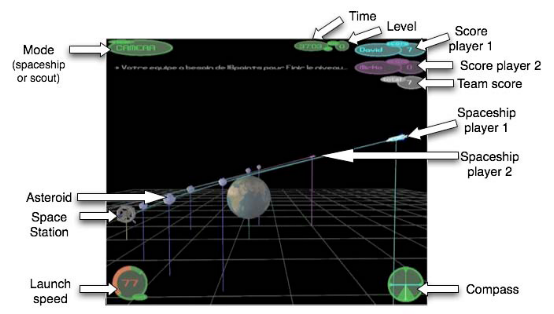
\includegraphics[width=0.9\textwidth]{image4.png}
        \caption{Snapshot of the SpaceMiner Game}
        \label{spaceminer}
\end{figure*}

\paragraph{Variables}

Task performance was measured by the score reached by the two subjects after
three situations. The effort of mutual modeling was measured as the ratio of
time that players would spend in the scout mode (divided by total time), which
is the time during which players are not performing their own actions but
monitoring their partner's actions.

In order to evaluate m°(A,B) during the task, we used two questionnaires (Figure
4) that were displayed during each of the three games, as a transparent layer
appearing over the game display. The first questionnaire concerned the player’s
intended actions. The second questionnaire asked each player about what he
thought her or his partner was intending to do. Some answers were identical in
both questionnaires (like “adjusting a shot”) while others were reversed ("to
guide my partner" versus "to guide me"). We chose this subjective measure of
accuracy (∆ M(A,B), M(B,B)) rather than an objective measure (i.e. model (A,B)
is compared to B's next action) because some the activities proposed by the
questionnaire were not observable by the environment (e.g. establishing a
strategy). We counted M°(A,B,activity,gamei) as the number of common answers
between questionnaires M(A,B) and M(B,B) in each game and computed the average
value a across the 3 games.


Figure 4: M(A,A) and M(A,B) questionnaires in SpaceMiners (translated from French)

\paragraph{Results}

Grounding criterion. The grounding criterion was high: the correlation between
M°(A,B) and task performance was 0.42, p = 0.05. Pairs with an accurate mutual
model reached higher scores. A regression analysis confirmed the positive and
significant relation between group performance and mutual modelling accuracy (β
=54, p = .02).

Study-specific questions. The awareness tool permitted higher group performance,
but it did not improve the accuracy of the mutual model. Since teams were free
to use the awareness tool or not (the 'scout' mode), we performed a post-hoc
split of players depending on how much time they used it. The split point was
the mean of time spent in the scout mode and it led to the constitution of two
groups made up of 12 individuals “short time in scout mode” and 24 individuals
“long time in scout mode”. A two-way analysis of variance conducted on these
contrasted groups revealed that pairs in the awareness condition who spent more
time in the scout mode reached higher levels of M°(A,B)(F = 8.02, p = 0.015). Of
course, a post-hoc split does not support a causal direction. An alternative
explanation could be that good modellers are more social and hence appreciate
the awareness tool.

Symmetry question. We computed intra-class correlation as described by Kenny et
al. (1998) from the answers to the cross-questionnaires. Considering all pairs
in both conditions, we found a positive and significant correlation (r = .38, p
< .05) between M°(A,B) and M°(B,A). Interestingly, this was higher in the
control group (r = 0.44) than in the experimental group (r = 0.24). Actually, ∆
(M°(A,B),M°(B,A)), i.e. the absolute differences between the models accuracy,
was not significantly different with or without the awareness tool ( F [1,13]=
0.144, p > 0.5). This result could be explained by the fact that the players
without awareness tools communicated more.

We cannot answer the triangle questions since this study was conducted with
pairs-

\paragraph{Discussion}

How to interpret a correlation of 0.38 between M°(A,B) and M°(B,A)? If it was
null, modelling would be interpreted as an individual process that varies
according to personality traits or cognitive skills: some persons tend to model
more accurately their peer while others don't care or can simply not. If the
correlation was close to 1, we could conclude that the modelling accuracy is an
emergent property of teams since there would be low probability that, by chance,
low accurate modellers are paired with accurate modellers and conversely. Our
correlation is between these two extremes but the very notion of significant
intra-class correlation tend to indicate that one may not consider peers as
independent subjects, which is an argument for the 'interaction' hypothesis
(H3). 


\bibliographystyle{abbrv}
\bibliography{biblio}



\end{document}

